\chapter{Metric Imitation for Efficient Distance Computation}
\label{ch:mi}
%%%%%%%%% TITL
%%%%%%%%% BODY TEXT

% {\bf Luc The paper only consists of text so far. A sketch of the 
% strategy early on may be helpful to explain the idea, but also to
% make it look less boring.}
The problem of computing good metrics is of great theoretical and
practical interest in information processing. Applications include
clustering~\citep{metric:nips03, metric:clustering:12}, image
annotation~\citep{tagprop:iccv09},
retrieval~\citep{local_distance:iccv:07, ml:fast:search:09},
classification~\citep{eigenface:pami97, local_distance:iccv:07,
  max:margin:knn}, among others.  It is often addressed by metric
learning~\citep{pairwise:metric:IJCAI09, large:scale:metric:cvpr12,
  tagprop:iccv09, max:margin:knn, qin:bmvc14}, with great success in
the past years. The drawback of metric learning is that it requires
some form of human annotation (\eg full category
labels~\citep{eigenface:pami97, local_distance:iccv:07, max:margin:knn,
  mlrank:10}, pairwise constraints~\citep{pairwise:metric:IJCAI09,
  ml:fast:search:09, large:scale:metric:cvpr12,
  fetlearn:convex:pami14}), which is expensive to acquire.

To address this problem, this paper aims to learn good metrics for cheap features without
using human annotation. We draw inspiration from transfer learning and
propose a novel approach, coined Metric Imitation (MI). 
MI takes state-of-the-art, off-the-shelf features as source features (SFs) and cheap features 
as target features (TFs) to learn good
metrics for the TFs by imitating the metrics computed
over the SFs. MI is a general framework and can at least
be applied to: 1) efficiently learning good TF metrics when
SFs are more powerful than TFs, but are computationally more expensive
and/or more memory-hungry; and 2) creating good metrics for TFs when SFs
contain privileged information but are not available at testing time. 


% in two manners: 1) perform normal
% distance measures (\eg L2 distance) on sophisticated,
% judiciously-designed (-learned) features
% (SFs)~\citep{objectbank:nips10, siftllc:cvpr10, fisher:eccv10,
%   super:coding:eccv10, middle:feature:cvpr10, rep:learn:pami13,
%   fetlearn:convex:pami14, Decaf:icml2014}; 2) using machine learning
% techniques to learn better metrics~\citep{pairwise:metric:IJCAI09,
%   large:scale:metric:cvpr12, tagprop:iccv09, max:margin:knn,
%   qin:bmvc14}, known as Metric Learning
% (ML)~\citep{metric:survey:12}. The two lines of research are sometimes
% coupled and both have enjoyed a huge success in the past years.
% However, they both have limitations. SFs are often very
% high-dimensional (tens of thousands dimensions, \cf
% Table~\ref{table:dim}), making metric computation inefficient,
% especially for applications with limited memory and time budget. ML is
% able to learn powerful metrics over cheap, low-dimensional features
% (CFs), but it often requires some form of human annotations (\eg full
% category labels~\citep{eigenface:pami97, local_distance:iccv:07,
%   max:margin:knn, mlr:10}, pairwise
% constraints~\citep{pairwise:metric:IJCAI09, ml:fast:search:09,
%   large:scale:metric:cvpr12, fetlearn:convex:pami14}), which is
% expensive to acquire, and jeopardizes the scalability of the system.

% To address these problems, this paper aims to learn good metrics over
% CFs without using human annotation. To achieve this goal, we propose a
% novel route to ML. The philosophy is to let the common metrics (\eg
% L2) computed over SFs, which are often able to yield satisfactory
% results but expensive to compute, supervise the metric learning
% process of CFs. This results in a transformation of CFs, under which
% CFs can generate better distance metrics than common ones (\eg
% L2). Specifically, the method works as follows: 1) quantifies the
% neighborhood properties defined over SFs into manifold geometries; 2)
% transfers the manifold to the domain of CFs; 3) learns a
% transformation of CFs so that the transferred manifold can be
% approximated as close as possible in the transformed space of CFs.  By
% doing this, the neighborhood properties of data computed over SFs is
% preserved in the transformed space of CFs, \ie close neighbors are
% still close. Put it in another word, the behavior of SFs is imitated
% by transformed CFs. The method is coined Metric Imitation (MI).

MI comes out of a marriage of advances in metric learning and transfer
learning. On the one hand, metric learning now is able to learn good
metrics over general features for specific tasks~\citep{metric:survey:12}, with human
supervision.
%  On the other hand, great advance has been made in feature representation,
% leading to a smorgasbord of sophisticated
% features~\citep{objectbank:nips10, siftllc:cvpr10, fisher:eccv10,
%   super:coding:eccv10, middle:feature:cvpr10, Decaf:icml2014}, which
% is able to produce good results even under common distance metrics
% (\eg L2). 
On the other hand, transfer learning can now transfer knowledge (often
classifiers) learned in one domain to
another~\citep{tl:survey}, for which no further human supervision is
necessary. Observing both developments then begs the question whether
metrics can be computed over one feature (\ie SFs) to then be
transferred to the domain of another feature (\ie TFs) and
automatically supervise the metric learning process there. 
In this paper, we demonstrate this for several vision tasks. The main
advantages of the method are: 1) it performs in an unsupervised
manner, i.e. without human annotation; 2) it can be efficient as only
TFs are needed during test time; 3) it can inject domain knowledge
carried through SFs to TFs for metric computation.  

The metric is learned in the framework of Mahalanobis distance
learning, \ie a linear mapping function of TFs is learned and applied
prior to performing the Euclidean distance metric. Specifically, the
method works as follows: 1) it translates the properties of metrics
computed over SFs into manifold geometries; 2) it transfers the
manifold to the domain of the TFs as view-independent properties; and
3) it learns a mapping function of the TFs so that the transferred
manifold is approximated as well as possible in the transformed
space. By doing this, the \emph{neighborhood properties} of data computed
over the SFs are preserved in the transformed space of TFs, \ie close
neighbors are still close. The reason for ensuring this is that
neighbors search is crucial in many vision applications,
such as clustering, retrieval, and classification.

% The only
% assumption of MI is that the mimiced metric should be better than the
% mimicing metric from the begining.
% Below, the procedures for training and testing are outlined. 

% Given a set of training images (without labels), the training of MI
% proceeds as follows: 1) it computes SFs and TFs for all training
% images; 2) it computes a standard metric (L2 distance in our
% implementation) over SFs and build up a manifold out of the metric to
% reflect the `intrinsic' neighborhood properties of input images; 3) it
% transfers the manifold to the domain of TFs and learns a mapping
% function for TFs so that the transferred manifold can be approximated
% as well as possible in the mapped space. A linear transformation is
% employed for the sake of efficiency. At testing time, MI works as
% follows to compute a metric over TFs: 1) compute TFs for test images;
% 2) perform the linear mapping to TFs corresponding to the learned
% mapping function; and 3) compute the Euclidean metrics over the mapped
% TFs. Hence, at testing time the only extra computational burden is a
% linear projection, which is very efficient especially for
% low-dimensional features.


%The whole pipeline of MI is shown in Fig.~\ref{fig:MI}.

% The goal of MI is different from ML, not ... , but to obtain a better
% metric for cheap, low-dimensional features without using human
% annotation. 

In accordance with our previous remarks, the usability of MI is
validated in two scenarios of metric learning: 1) compute good metrics for cheap features; 
and 2) transfer privileged information. For the first scenario,
MI was tested on instance-based object retrieval using the INRIA
Holiday dataset~\citep{hamming:embedding:08} and the UKbench
dataset~\citep{ukbench:cvpr06}, and on category-based image retrieval
and image clustering using four other datasets:
Scene-15~\citep{lazebnik:cvpr06}, CUReT-61~\citep{CUReT-61},
Caltech-101~\citep{FeiFei2004}, and
Event-8~\citep{event8}. % These 4 datasets are popular for testing the
% recognition of scenes, textures, objects, and events, resp.
Three sophisticated, high-dimensional features were used as the SFs:
object-bank~\citep{objectbank:nips10}, SIFT-llc~\citep{siftllc:cvpr10},
and the CNN feature~\citep{deep:bmvc14}, and three general, cheap
features used as the TFs: GIST~\citep{gist}, LBP~\citep{lbp}, and
PHOG~\citep{phog}. Extensive experiments show that MI consistently and
significantly outperforms the metrics computed directly over the same
TFs, while getting very close to the metrics from the computationally
more expensive SFs in some cases. For the second scenario, MI was
evaluated on example-based image super-resolution. Patches of
high-resolution images, which are not available at testing time, are
used as SFs and patches of low-resolution images as TFs. Experiments
show that MI is able to improve the performance of $k$-NN-based methods
for image super-resolution.

% Our main contributions are threefold: 1) we propose Metric Imitation
% as a novel approach to learn good metrics under weak supervision; 2)
% we develop a solution for this approach via manifold transfer; and 3)
% we apply the method to multiple vision tasks. The code of our method
% will be made publicly available upon the acceptance of the paper.

% The paper is structured as follows. Sec.\ref{sec:rel} discusses
% related work. Sec.\ref{sec:app} describes the approach, which is
% validated by experiments in Sec.\ref{sec:exp}. Finally,
% Sec.\ref{sec:con} concludes the paper. 

%%%%%%%%%%%%%%%%%%%%%%%%%%%%%%%%%%%%%%%%%%%%%%%%%%%%%%%%%%%%%%%%%%%

\section{Related Work}
\label{sec:rel}

Our method is generally relevant to Metric Learning, Feature
Embedding, and Transfer Learning.

\subsection{Metric Learning}
% {\bf Luc You now use ML not only to mean Machine Learning, but ale
% Metric Learning. That only causes confusion and must be changed… I
% removed ML here, but maybe ML still means metric learning elsewhere
% in the paper.}
There has been a great deal of research devoted to metric learning
to tune distance functions  with human supervision. % - to particular 
% tasks such as face/person identification~\citep{ml:face:09,
%   ml:pedestrain:11}, classification~\citep{max:margin:knn}, retrieval
% (ranking)~\citep{ml:fast:search:09, mlr:10}, and
% tracking~\citep{ml:tracking:06}.
Typically, metric learning methods 
follow as guiding principle to learn a mapping that shrinks the
distances between similar objects, while expanding the distance between 
dissimilar objects. 
% Constraints between pairs of distances can be gathered from
% click-through feedback or in fully supervised settings, it can be
% inferred so that points in the same class have smaller distances to
% each other than to points in different classes.
% The methods mainly differ in the manner how similar points are defined
% (annotated), and the objective functions defined (often
% task-specific). 
Since a comprehensive overview is beyond the scope of this paper, we
summarize the most relevant ones according to the types of annotation
used. Readers are referred to~\citep{metric:survey:12}
for a survey.

\textbf{Class label} is one of the most popular annotation types for
metric learning. 
% Xing \etal~\citep{metric:nips03} define the good
% neighbors as all points sharing the same class, and learn the metric
% by mapping each class into a ball of fixed radius while maximizing the
% distances between points from different classes.  
Notable examples include Neighborhood Component Analysis (NCA)~\citep{NCA:2004}, 
Collapsing Classes (CC)~\citep{class:clapse:nips05} and Large-Margin 
Nearest Neighbors (LMNN)~\citep{max:margin:knn}. NCA maximizes the expected 
number of correctly retrieved points under a stochastic neighbor selection
rule. CC optimizes a similar stochastic neighbor selection rule while
attempting to collapse each class to a single point. The idea enforces
more regularity on the output space than NCA and leads to a convex
optimization problem, but the assumption that entire classes can be
collapsed to distinct points rarely holds in practice.
LMNN~\citep{max:margin:knn} relaxes this strong assumption by defining
target neighbors as the $k$ closest samples in the same class, and
maximizes margins between distances to target neighbors and to other
points.

\textbf{Pairwise Constraints} correspond to another popular type of
annotation used in metric learning, in which similar (dissimilar)
pairs of objects are indicated. Earlier work by Xing
\etal~\citep{metric:nips03} formulates the clustering problem as a
semi-definite programming task under similarity and dissimilarity
constraints. With similar annotations, Davis
\etal~\citep{ml:information:07} tackle the metric learning problem with
an information theoretic approach, namely by minimizing the
Kullback-Leibler divergence between a learned and a prior matrix,
expressing the pairwise constraints. Guillaumin
\etal~\citep{ml:face:09} offer a probabilistic view on learning
distance metrics with pairwise constraints and solve the problem by
MAP. Following the spirit of~\citep{ml:information:07, ml:face:09},
Kostinger \etal \citep{large:scale:metric:cvpr12} present the KISS
framework by formulating the problem as a likelihood ratio test, which
avoids complex optimization problems.  

While all these methods perform well, human annotations have to be
provided. As a result, methods requiring weaker or no supervision are
desired. Our method offers this by learning metrics over
cheap features by imitating the standard metrics computed over other, sophisticated 
off-the-shelf features, which either contain privileged information or are more
useful for the tasks at hand but too computationally expensive.

% Viewing the objective of ML in a
% higher level, McFee and Lanckriet~\citep{mlr:10} learns good metrics by
% optimizing directly over ranking measures, such as AUC, Average
% Precision within the framework of structure learning. 

% learning framework, we can view metric learning algorithms as learning
% a linear transformation to be applied to the data. 
% Which basically shrink the distance between images of pairs of similar
% objects and expand the distance between pairs of dissimilar objects.

% Knn based approaches as mahalanobis metric learning have
% ... improvements have been observed for tracking, image retrieval,
% face identification, clustering or person re-identification.


% [Joint learning of discriminative prototypes and Large Margin Nearest
% neighbor classifiers]

\subsection{Embedding}
There is a great deal of work about embedding for nonlinear
dimensionality reduction, with the philosophy that many
high-dimensional data can be characterized by a low-dimensional
nonlinear manifold. The methods broadly fall into two categories:
those providing a mapping function for out-of-sample extension and 
those just offering a visualization. We will briefly overview the 
methods which provide mapping functions. Embedding methods proceed 
mainly in two steps: 1) quantify manifold properties (local geometry); 
and 2) seek a low-dimensional space so that the learned properties 
are mostly preserved. A large range of manifold properties have been
considered. For instance, Multi-dimensional
Scaling~\citep{MDScaling:08} and its extension Isomaps~\citep{isomap:00}
are designed to capture and preserve pairwise distances between
points. Locally-linear embedding (LLE)~\citep{lle:science00,
  NPEmbedding:iccv05} computes the local linearity of the
manifold and attempts to preserve that in the low-dimensional space.
Laplacian Eigenmaps (LapEigen)~\citep{eigenmaps:nips01}, and Hessian LLE
(HLLE)~\citep{hlle}. % , and Local Tangent Space Analysis
% (LTSA)~\citep{ltsa}
proceed in a similar manner as LLE does, but the
properties captured are the locality of the manifold, and the local 
curvature of the manifold.
%  , and the coordinates in local tangent space, resp
Due to space limitations interested readers are referred to the
comparative overview in~\citep{embedding:overview:09}.

Our approach draws inspiration from and extends the traditional
embedding methods. % by taking full advantage of progress in feature
% representations. We learn the manifold properties with powerful but
% expensive features, and then transfer this manifold to learn a
% mapping function for weaker, but much cheaper features.
The method 
imitates the manifold properties obtained from SFs by learning a 
transformation for the TFs, trading off a slight drop in precision 
against a significant gain in efficiency. The method also avoids 
feature embedding in the high-dimensional space of SFs, which is 
time-consuming.

% Another group of techniques for efficient nearest neighbors are
% hashing methods~\citep{ukbench:cvpr06, shashing:nips09,
%   mlhashing:icml11}. The methods focus on finding mapping functions
% from high-dimensional representations to compact binary codes for
% efficient search. MI is different mainly because it lifts the need to
% compute high-dimensional features during the test phase.

% One inherent drawback of
% Mahalanobis metric learning based methods is that the k-NN search in
% high-dimensional spaces is time-consuming, even on moderate sized
% datasets. For real-time applications with limited time budget and
% memory budget this is even more critical. To alleviate this problem,
% different solutions have been proposed that focus on low dimensional
% embeddings. This can be done by applying locality sensitive hash
% function [16] or learn a low-rank Mahalanobis distance metirc [29]
% that performs dimensionality reduction.

% Special data structures as metric ball trees have been introduced to
% speeed up nearest neighbor search. Unfortunately, there is no
% significant time gain for high dimensional space.


\subsection{Transfer Learning and Domain Adaptation}
Our method also is akin to transfer learning.  Transfer
learning addresses the problem of transferring the knowledge learned
in a source domain to a different target domain. Successful
applications in vision include knowledge transfer from one data source
to another (\eg videos to images)~\citep{tl:kernel:11, DA:iccv11,
  DASA:iccv13} and knowledge transfer from known classes to unseen
classes~\citep{tl:attribute:09}. The difference between such work and
ours is in the form of the knowledge. These methods transfer
definitions of classes (learned classifiers) to a new domain where few
or no training data is available, by reducing the discrepancy from
source domain to target domain. Our goal, however, is to transfer the
manifold structure from our source domain to a target domain to
imitate the metrics computed in the source domain, where features in
the source domain are kept intact. This distinction leads to 
different algorithms and applications.

% The closest work to ours would be the work~\citep{DA:iccv11,
%   DASA:iccv13} where \emph{subspace alignment} is used for domain
% adaptation. In these work, they reduce the discrepancy between the
% source domain and the target domain by moving closer the source and
% target subspaces.  or finding common intermediate subspaces for the
% source features and target features. 



\section{Metric Imitation}
\label{sec:app}
In this section, we will introduce Metric Imitation (MI) in detail. 
Like most metric learning or embedding methods, MI operates in
two modes: training and mapping. Training learns
the projection transformation matrix $A$ guided by the transferred 
manifold, while `mapping' performs the learned transformation for 
better distance metrics during testing.

The generic problem of MI can be summarized as follows. Given a set of
$n$ training images $\mathcal{D} = \{I_1, I_2, ..., I_n\}$, and their
corresponding SFs $\mathcal{D}_s = \{ \efet{x}_1, \efet{x}_2, ...,
\efet{x}_n\} \in \mathbb{R}^{m \times n}$ and TFs $\mathcal{D}_c = \{
\cfet{y}_1, \cfet{y}_2, ..., \cfet{y}_n\} \in \mathbb{R}^{q \times n}$
(often $q \ll m$), the goal is to find a transformation matrix $A \in
\mathbb{R}^{q \times q}$ that maps the $n$ TFs $\cfet{y}$'s to $n$
transformed points $\bar{\mathcal{D}}_c = \{ \ctfet{y}_1, \ctfet{y}_2,
..., \ctfet{y}_n\}$, where $ \ctfet{y}_i = A^T\cfet{y}_i$. The guiding
principle of the learning is to approximate the manifold defined by
all $\efet{x}$'s by the manifold defined over all $\ctfet{y}$'s.  Note
that the transformation matrix $A$ can be a low-rank matrix for the
purpose of further dimension reduction. We force it to be a full-rank
matrix, as the dimensionality of $\cfet{y}$ is itself quite low. 


\subsection{Training}
The training part comes with two components: learning the intrinsic
manifold over the input $\efet{x}$'s, and learning a transformation 
that has to be applied to the $\cfet{y}$'s such that the `intrinsic' 
manifold is approximated as closely as possible in the learned space
of $\ctfet{y}$'s. 

\begin{enumerate} [leftmargin=4.5mm]
\item \textbf{Learning the intrinsic manifold over SFs}: the aim of
  this step is to capture the `intrinsic manifold', i.e. the manifold
  underlying the input data. Since visual data is highly nonlinear, 
  its global manifold layout tends to be captured better by local 
  properties, such as Local Linear Embedding (LLE)~\citep{lle:science00}, 
  Laplacian Eigenmaps (LapEigen)~\citep{eigenmaps:nips01}, or Hessian 
  LLE (HLLE)~\citep{hlle}. Compared to methods for global properties, such
  as Isomap~\citep{isomap:00}, local ones have several advantages. They
  typically yield better results, and are faster when advantage is taken 
  of matrix sparsity. Local methods share that they first induce a
  local neighborhood structure over the input data, and then quantify
  the corresponding local properties over the neighborhood
  structure. In these methods, the learned manifold is used for
  dimensionality reduction~\citep{lle:science00, eigenmaps:nips01,
    hlle}. However, we use the manifold as a guide to learn a
  transformation of other features, which are much cheaper to compute
  and store, so that the learned manifold is approximated with good
  precision in the transformed space. Below come the two steps of
  the learning.
 
 \begin{enumerate} [leftmargin=5mm]
 \item Constructing an adjacency graph: by taking each image $I$ in
   $\mathcal{D}$ as a node, the adjacency graph $G = (\mathcal{D},
   \mathcal{E})$ can be constructed in the following way: a directed
   edge from node $i$ to node $j$ is added, \ie $e_{ij}=1$, if $I_j$
   is among the $K$ nearest neighbors of $I_i$. The features in source
   domain $\efet{x}$ are used to compute the neighbors under the $L_2$
   distance, but any distance measure can be applied. The global
   structure of the nonlinear manifold is captured by the interaction
   of these overlapping local structures. The largest connected
   component is used for further analysis if the graph is not fully
   connected.
   
 \item Quantifying the local properties of the manifold: The local
   properties (relations) of the manifold can be quantified in a variety
   of ways, including local linearity as in
   LLE~\citep{lle:science00, NPEmbedding:iccv05}, local pairwise
   distance as in LapEigen~\citep{eigenmaps:nips01}, local `curviness' as in
   HLLE~\citep{hlle}, etc. Here, we use two of
   the most representative ones: local linearity and local pairwise
   distance. For the reason of efficiency, their linear variants are
   used.
   
   \begin{itemize} [leftmargin=4mm]
   \item LLE~\citep{lle:science00} assumes that the manifold is locally
     linear, \ie a data point $\efet{x}_i$
     is characterized by encoding $\efet{x}_i$ as a linear combination
     $W_i$ (reconstruction weights) of its $k$ nearest neighbors
     $\efet{x}_{ij}$. The weights $W$ are learned by minimizing the
     following reconstruction error: 
     
     \begin{equation}
       \label{eq:lle:error}
       \begin{aligned}
         \underset{W} {\text {minimize }} \sum_{i=1}^n \| \efet{x}_i - \sum_{j=1}^n W_{ij} \efet{x}_j \|^2 \\
        \text{s.t. }  \sum_{j=1}^n W_{ij}=1 
       \end{aligned}
     \end{equation}
     where $W_{ij}$ is only allowed to have non-zero value if
     $e_{ij}=1$. 
% Interested readers are referred
%      to~\citep{lle:science00} for how to solve the equation.

   \item LapEigen~\citep{eigenmaps:nips01} characterizes the local
     manifold structure by encoding the pairwise distances between
     close neighbors. The neighbors are defined also over the graph
     $G$. The weight matrix $W$ is defined as a Gaussian kernel
     function over the distance of neighboring nodes to reflect the
     proximity of data points: 
 
     \begin{equation}
       \label{eq:lap:wt} 
       w_{ij} = \begin{cases}  \exp{ -\frac{ \| \efet{x}_i - \efet{x}_j \| ^2} {2\sigma^2}}, &\text{if } e_{ij}=1  \\
                               0          &\text{otherwise}
                \end{cases}
     \end{equation}
     where $\sigma$ modulates the decreasing rate of $W$ with the
     distance.
   \end{itemize}

   Metric Imitation (MI) learns the structure of the manifold underlying
   the $\efet{x}$'s and describes its local properties through the weight 
   matrix $W$. The learned $W$ is then transferred to the domain of the
   $\cfet{y}$'s. There a linear mapping is learned, i.e. a matrix $A \in 
   \mathbb{R}^{q \times q}$ to be applied to the $\cfet{y}$'s in order to 
   mimic corresponding manifold characteristics:
   1) for LLE, a transformation is learned for $\cfet{y}$'s so that
   all mapped data points $\ctfet{y}$'s are reconstructed well from their
   neighbors (defined in graph $G$) with the learned reconstruction
   weight $W$; 2) for LapEigen, MI learns a projection so that all
   nearby points in the space of the $\efet{x}$'s are still nearby
   points in the mapped space of the $\ctfet{y}$'s.

   \end{enumerate}

 \item \textbf{Approximating the manifold by using the TFs}: with the
   learned manifold property $W$ from SFs (in the manner of LLE or
   LapEigen), the aim of this step is to compute a linear projection
   matrix $A$ for TFs so that the manifold properties learned over the
   SFs are preserved as much as possible in the transformed space. 
   Specifically, MI minimizes the following cost
   function:
   \begin{equation}
     \label{eq:mapping:cost}
         \begin{aligned}
         \underset{\ctfet{y}} {\text {minimize }}  \sum_{i=1}^n  \| \ctfet{y}_i - \sum_{j=1}^n W_{ij} \ctfet{y}_j \|^2. \\
         \end{aligned}
   \end{equation}
   The cost function is very similar to that in Eq.\ref{eq:lle:error},
   but here the weight matrix $W$ is fixed and the optimization is
   performed over the $\ctfet{y}$. For the sake of efficiency,
   $\ctfet{y}$ is constrained to be a transformed version of
   $\cfet{y}$ by a linear transformation: $\ctfet{y} = A^T\cfet{y}$.
   % This optimization problem is very similar to the embedding problems
   % in~\citep{lle:science00, eigenmaps:nips01, NPEmbedding:iccv05} to
   % reduce feature dimensionality, while here a transformation of a
   % feature $\cfet{y}$ is learned to best approximate the
   % manifold geometry $W$ injected from another feature
   % $\efet{x}$.  
According to the induction of~\citep{NPEmbedding:iccv05}, solving Eq.\ref{eq:mapping:cost} can be reduced to solving
   the following generalized eigenvector problem:
   \begin{equation}
     \label{eq:mapping:cost2}
         \begin{aligned}
           YMY^T \vect{a} = \lambda YY^T \vect{a},
         \end{aligned}
   \end{equation}
   where  
 \begin{align*}
     & Y = (\cfet{y}_1, ..., \cfet{y}_n), \\
     M &= (I-W)^T (I-W),   \\
     &I = diag(1, ..., 1).  
\end{align*}
Solving Eq.\ref{eq:mapping:cost2} leads to $q$ eigenvectors
$\vect{a}_1, ..., \vect{a}_q$, with eigenvalues ordered from the
smallest to the largest.  Thus, the embedding is performed as:

\begin{equation}
  \label{eq:embedding}
  \cfet{y} \to \ctfet{y} \doteq A^T \cfet{y}, 
\end{equation}
where the projection matrix $A = (\vect{a}_1, \vect{a}_1, ...,
\vect{a}_{q})$.
\end{enumerate}

%========================================================================

\subsection{Mapping}
During the test phase, MI only computes the TFs $\cfet{y}$'s, for the
test images, and then computes the distance metric over them with the 
learned projection matrix $A$:
\begin{equation}
  \label{eq:tdis}
  d(\cfet{y}_i, \cfet{y}_j) = \|\ctfet{y}_i - \ctfet{y}_j\|^2 = \|A^T\cfet{y}_i - A^T\cfet{y}_j\|^2, 
\end{equation}
which is then used for the task at hand. Computing the Euclidean
distance in this transformed space equals to computing the following
Mahalanobis distance function in the original feature space: 
%
 \begin{align}
\label{eq:mdis}
  d(\cfet{y}_i, \cfet{y}_j) = &(\cfet{y}_i - \cfet{y}_j )^T H (\cfet{y}_i - \cfet{y}_j)  \nonumber \\
                           = & (\cfet{y}_i - \cfet{y}_j )^T A^TA (\cfet{y}_i - \cfet{y}_j).  
 \end{align}
%
 The form of Eq.\ref{eq:tdis} is preferred to that of
 Eq.\ref{eq:mdis}, because many approximate, fast nearest neighbor
 techniques have been developed for the euclidean metric. Since the
 space is learned to preserve the neighborhood properties of the
 `intrinsic' manifold, superior performance over common metrics on
 original TFs is expected.  Although our mapping and the embedding for
 dimensionality reduction are similar technically, they serve totally
 different purposes. The advantages of MI over the embedding for
 dimensionality reduction of SFs are twofold: 1) computationally more
 efficient, as SFs are not needed by MI during testing, and 2) more
 robust, as fewer parameters are needed to learn the projection, as $q
 \ll m$. The advantage of MI over the embedding for TFs is that the
 `privileged' information in the source domain is injected into the target
 domain at little extra cost.



% \subsection{Implementation Details} 
% 1. if cheap feature linear dependent, then either singular value decomposition or add a little bit noise to avoid any problem. 


%%%%%%%%%%%%%%%%%%%%%%%%%%%%%%%%%%%%%%%%%%%%%%%%%%%%%%%%%%%%%%%%%%%
%%%%%%%%%%%%%%%%%%%%%%%%%%%%%%%%%%%%%%%%%%%%%%%%%%%%%%%%%%%%%%%%%%%

\section{Experiments} 
\label{sec:exp}

We evaluated Metric Imitation (MI) in the two aforementioned
scenarios: 1) learning of good metrics when the source
features (SFs) are more powerful but computationally more expensive
than the target features (TFs); 2) when SFs contain privileged
information but are not available during test time. For the first, MI
was evaluated on image clustering, category-based image retrieval, and
instance-based object retrieval. For the second, MI is evaluated on
example-based super-resolution. For all experiments of these four
tasks, MI uses identical parameter settings: the size of the
neighborhood $K$ was set to $40$ and $\sigma$ in Eq.\ref{eq:lap:wt}
was set to the mean of the $L_2$ distance between all feature vectors $\|
\vect{x}_i - \vect{x}_j \|^2, $ where $i, j \in \{1, ..., n \}$. These
values have been set empirically, but our experiments show that MI is
not very sensitive to these choices. If needed, a cross-validation on
hold-out sets can be considered.


%=================================================================

\subsection{Image Clustering}
\label{sec:img:clustering}
As the amount of image data is on a rampant increase, unsupervised 
methods to group objects into semantically relevant clusters are in 
great demand. Such clustering is one of the core problems in modern
computer vision. In this section, we apply MI to image clustering.

\textbf{Datasets}: The following four popular datasets are used:
Scene-15~\citep{lazebnik:cvpr06}, CUReT-61~\citep{CUReT-61},
Caltech-101~\citep{FeiFei2004}, and Event-8~\citep{event8}. They contain
$4585$ images of $15$ classes of general scenes, $5612$ images of $61$
texture classes, $8677$ images of $101$ object classes, and $1574$
images of $8$ classes of sports events, respectively.

\textbf{Features}: In order to sufficiently sample the space of
possible features, three different SFs and three different TFs are
chosen. The SFs are: SIFT-llc~\citep{siftllc:cvpr10},
object-bank(OB)~\citep{objectbank:nips10}, and the CNN
feature~\citep{deep:bmvc14}. The chosen TFs are: GIST~\citep{gist},
LBP~\citep{lbp}, and PHOG~\citep{phog}. They were chosen because they
are popular in the community, come with available code, and are based
on different underlying techniques. Another more important reason is
that the three SFs are representatives of the state-of-the-art
features but computationally expensive (relatively), and the three TFs
are low-dimensional and computationally very cheap.

SIFT-llc is a representative image representation based on local
descriptors, which utilizes the locality constraints to encode local
descriptors and integrates the results by max-pooling.  The CNN
feature~\citep{deep:bmvc14} is obtained by vectorizing the
convolutional results of the deep convolutional neural
network~\citep{deepnet:nips12}, which is trained on the ImageNet
dataset. OB performs object detectors as filters and collects the
response of these semantic filters over an image. The features were
computed as follows.
SIFT-llc\footnote{\url{http://www.ifp.illinois.edu/~jyang29/LLC.htm}}
and OB\footnote{\url{http://vision.stanford.edu/projects/objectbank}}
were computed with their default parameters in the authors'
implementations. For the CNN feature, the MatConvNet
package~\citep{MatConvNet} was used with a pre-trained
CNN model. The convolutional results at layer $16$ were stacked as the CNN
feature vector, with dimensionality $4096$.  GIST was computed with
only one cell. For LBP, the uniform one was used with PCA for further
dimensionality reduction. For PHOG, the 2-layer pyramid was used. The
dimensionalities of the six features are listed in Table~\ref{table:dim},
from which it is evident that the TFs are much lighter and efficient
to compute and handle, in line with the aims of MI.

\textbf{Evaluation}: We follow~\citep{comp:ijcv09, dai:cvpr10, dai:ensemble:eccv12}
and used Purity (bigger=better) for evaluation.  It measures how pure
the discovered clusters are according to the ground truth class
labels. Spectral Clustering was used on top of MI for the
clustering. We compared to Spectral Clustering with the SFs and TFs as
inputs. The K-means algorithm was also tried, but it generally
produces similar or poorer results than Spectral Clustering.  As
suggested in~\citep{dai:ensemble:eccv12}, we use the $\chi^2$ distance
for LBP and PHOG, and the Euclidean distance for GIST. Euclidean
distance is used for all the SFs.

\textbf{Results:} $50\%$ of the images (without labels) were used for
training and the rest used for testing. Table~\ref{tab:clustering}
lists the results of all methods on the four datasets over $5$ random
training-test splits. Due to space limitations only one type of TFs,
LBP, is listed here (same for the following experiments). GIST and PHOG generally yield similar trends than LBP, and
their outcomes are reported in the supplementary material. It is
expected to find that the SFs perform significantly better than the
TFs on image clustering. This allows MI to learn `useful' knowledge
from the SFs.  From the table, it is evident that MI is able to learn
a better metric for the TFs than the common, generic ones (\eg
$\chi^2$ and $L_2$). For instance, on Scene-15 MI improves the purity of
LBP from $0.36$ to $0.48$ if the CNN feature is used as the SFs and LapEigen is
chosen. On Event-8, MI improves the
purity of LBP from $0.38$ to $0.48$ when OB is used as the SFs
and LLE is used. Similar trends can
be observed across all datasets, all SFs, and the two ways of encoding
manifold properties. This shows that MI efficiently provides good
metrics for image clustering in general, and that the framework is robust to the
specific choices of its components.

% , except when the choices of the components are 
% very `unwise', \eg using GIST, a holistic feature, as the TFs to represent fine-grained texture classes. 

\textbf{Across classes}: In order to check the generality of MI, we
also tested MI in a wilder scenario, where training and test images
are from totally different classes. Half of the classes (floored to
the closest integer) were used for training and the rest of classes
used for testing, \ie $7$ classes used for training for Scene-15, $30$
for CUReT-61, $50$ for Caltech-101, and $4$ for Event-8.  All methods
run over $5$ random training-testing splits and the average results
are reported in Table~\ref{tab:clustering:across}. The table shows
that even when the training images and test images are from different
distributions, MI is still able to improve the performance over the
standard metrics of TFs. This suggests that MI is also able to work in
a fully unsupervised manner. This property is important, especially
for online applications where test data is not available beforehand.

% \begin{table}
%   \centering \small
%   \caption{The dimensionality of the features.}
%   \begin{tabular}{ccc|ccc}  
%    \multicolumn{3}{c|}{SFs}  & \multicolumn{3}{c}{ TFs}  \\   \hline
%     SIFT-llc & OB & CNN & GIST & LBP & PHOG  \\ \hline
%     21504   & 44604  & 43264 & 20    & 59    & 40     \\  
%   \end{tabular}
%   \label{table:dim} \vspace{-4mm}
% \end{table}

\begin{table}
  \centering \small \setlength{\tabcolsep}{.60em} 
  \caption{The dimensionality of the features.}
  \begin{tabular}{ccc|ccc}  
   \multicolumn{3}{c|}{TFs}  & \multicolumn{3}{c}{ SFs}  \\   \hline
    GIST  & PHOG & LBP &  CNN   & SIFT-llc  & OB      \\ \hline
    20   & 40  & 59     &   4096 &21504     & 44604              \\  
  \end{tabular}
  \label{table:dim} 
\end{table}

  
% \begin{table*}[!tb]
%   \centering \small
% $\begin{array} {ccccccccc}

%   \begin{tabular}{|c|} \hline
%        \\ 
%     Scene-15 \\  
%     CUReT-61 \\  
%    Caltech-101 \\
%    Event-8     \\   \hline
%   \end{tabular}


%   \begin{tabular}{||c|c|c|c||}
%     \hline
%      LBP & LLE & Lap & SIFT-llc \\
%      0.34  & 0.40  & 0.46  & 0.49   \\
%      0.29  & 0.44  & 0.46  & 0.39  \\
%      0.28  & 0.34  & 0.34  & 0.51 \\
%     0.34  & 0.50  & 0.41  & 0.60  \\ \hline
%   \end{tabular}

% \end{array}$
%   \caption{Purity of clustering by Metric Imitation (MI), where $50\%$ of the images are used for training and the rest for testing.}
%   \label{tab:clustering}
% \end{table*}


\begin{table*}[!tb]
  \centering \small \setlength{\tabcolsep}{.60em} 
  \caption{Purity of clustering by Metric Imitation (MI), where $50\%$ of the images are used for training and the rest for testing.}
  \begin{tabular}{c|c|ccc|ccc|cccc}
   & TFs & \multicolumn{2}{c}{\textbf{MI}} & SFs & \multicolumn{2}{c}{ \textbf{MI} } & SFs & \multicolumn{2}{c}{ \textbf{MI}} & SFs  \\   
  Lap  & LBP & LLE & Lap & SIFT-llc  & LLE & Lap & CNN &  LLE & Lap & OB     \\   \hline
    Scene-15 & 0.36  & 0.40  & 0.46  & 0.49    & 0.47  & 0.48  & 0.69    & 0.42  & 0.48  & 0.54 \\ 
    CUReT-61 & 0.33  & 0.44  & 0.46  & 0.39    & 0.33  & 0.41  & 0.60  & 0.31  & 0.37  & 0.44 \\ 
    Caltech-101 & 0.32  & 0.34  & 0.34  & 0.51   & 0.37  & 0.36  & 0.68       & 0.37  & 0.35 & 0.52    \\
    % Event-8 & 0.34  & 0.50  & 0.41  & 0.60  & 0.34  & 0.46  & 0.45  & 0.62  & 0.34  & 0.44  & 0.46  & 0.45 \\ \hline  Lap
    Event-8 & 0.39  & 0.46  & 0.46  & 0.57    & 0.47  & 0.47  & 0.82    & 0.48  & 0.48  & 0.46 \\  
  \end{tabular}
  \label{tab:clustering}
\end{table*}


\begin{table*}[!tb]
  \centering \small  \setlength{\tabcolsep}{.60em} 
  \caption{Purity of clustering by Metric Imitation (MI) across classes, where half of the classes are used for training and others for testing.}
  \begin{tabular}{c|c|ccc|ccc|cccc}
   & TFs & \multicolumn{2}{c}{\textbf{MI}} & SFs & \multicolumn{2}{c}{ \textbf{MI} } & SFs & \multicolumn{2}{c}{ \textbf{MI}} & SFs  \\   
    & LBP & LLE & Lap & SIFT-llc  & LLE & Lap & CNN &  LLE & Lap & OB     \\   \hline
     Scene-15    & 0.63  & 0.67  & 0.70  & 0.85  & 0.65  & 0.66  & 0.90    & 0.61  & 0.59  & 0.74 \\ 
    CUReT-61 & 0.62  & 0.62  & 0.64  & 0.65   & 0.66  & 0.69  & 0.77   & 0.51  & 0.58  & 0.68 \\ 
    Caltech-101 & 0.57  & 0.62  & 0.60  & 0.73  & 0.59  & 0.57  & 0.77     & 0.64  &0.63 &  0.70   \\ 
    Event8 & 0.70  & 0.72  & 0.74  & 0.80   & 0.70  & 0.72  & 0.89    & 0.75  & 0.73  & 0.80\\    \end{tabular}
  \label{tab:clustering:across}
\end{table*}


\begin{table*}[!tb]
  \centering \small  \setlength{\tabcolsep}{.60em} 
  \caption{The computational time (in seconds) of a full matrix of pairwise distance with different 
    features, where MI(X) denotes that Metric Imitation for feature X.   }
  \begin{tabular}{c|ccc|ccc|ccc}  
 &  \multicolumn{3}{c}{\textbf{SFs}}   & \multicolumn{3}{c}{\textbf{MI}} & \multicolumn{3}{c}{\textbf{TFs}}  \\ 
   & GIST   & PHOG &LBP &  GIST & MI  &  MI &   CNN & SIFT-llc & OB \\ \hline
 Scene-15 & 0.41    & 0.47 & 0.53  & 0.41     & 0.48 & 0.53 & 21.92 & 104.83  & 215.56   \\
 CURet-61  & 0.61  & 0.71 & 0.78    & 0.62    & 0.71 & 0.84 & 32.68 & 161.29  & 325.97   \\ 
 Caltech-101 & 1.51  & 1.73 & 1.96  & 1.51    & 1.75 & 2.01  & 78.67  & 388.01  & 796.86 \\ 
 Event-8  & 0.05    & 0.06 & 0.08  & 0.05   & 0.06 & 0.08    & 2.76 & 13.56  & 26.69  \\ 
  \end{tabular}
  \label{tab:time}
\end{table*}


\begin{table*}[!tb]
  \centering \small    \setlength{\tabcolsep}{.60em} 
  \caption{MAP of category-based image retrieval by MI, with $50\%$ images used for training and the rest for testing, and recall set to $0.1$.}
  \begin{tabular}{c|c|ccc|ccc|cccc}
   & TFs & \multicolumn{2}{c}{\textbf{MI}} & SFs & \multicolumn{2}{c}{ \textbf{MI} } & SFs & \multicolumn{2}{c}{ \textbf{MI}} & SFs  \\   
    & LBP & LLE & Lap & SIFT-llc  & LLE & Lap & CNN &  LLE & Lap & OB     \\   \hline  
   Scene-15  & 0.50  & 0.54  & 0.55  & 0.60   & 0.58  & 0.58  & 0.72   & 0.56  & 0.57  & 0.65 \\   
   CUReT-61  & 0.83  & 0.90  & 0.87  & 0.90  & 0.90  & 0.90  & 0.95 & 0.86  & 0.84  & 0.90 \\ 
   Caltech-101  & 0.35  & 0.39  & 0.38  & 0.57  & 0.41  & 0.41  & 0.79  & 0.40  & 0.40  & 0.60 \\  
   Event-8 & 0.44  & 0.53  & 0.52  & 0.70    & 0.53  & 0.55  & 0.89    & 0.51  & 0.50  & 0.60 \\   
  \end{tabular}
  \label{tab:class:retreval} 
\end{table*}


%\textbf{Performance of the Concatenation of EFs}


 \begin{table*}[!tb]
   \centering \small  \setlength{\tabcolsep}{.60em} 
\caption{MAP of category-based image retrieval by MI with the concatenation of LBP, GIST and PHOG (LGP) used as the TFs. 
    $50\%$ images are used for training and the rest for testing. Recall is set to $0.1$.}
  \begin{tabular}{c|c|ccc|ccc|cccc}
   & TFs & \multicolumn{2}{c}{\textbf{MI}} & SFs & \multicolumn{2}{c}{ \textbf{MI} } & SFs & \multicolumn{2}{c}{ \textbf{MI}} & SFs  \\   
    & LGP & LLE & Lap & SIFT-llc  & LLE & Lap & CNN &  LLE & Lap & OB     \\   \hline  
      Scene-15 & 0.52  & 0.60  & 0.61  & 0.60   & 0.64  & 0.64  & 0.72   & 0.62  & 0.63  & 0.65 \\ 
      CUReT-61 & 0.84  & 0.95  & 0.93  & 0.90    & 0.94  & 0.96  & 0.95    & 0.92  & 0.90  & 0.91 \\ 
      Caltech-101 & 0.42  & 0.48  & 0.46  & 0.57   & 0.51  & 0.51  & 0.79  & 0.48  & 0.48  & 0.59 \\ 
     Event-8 & 0.52  & 0.63  & 0.63  & 0.70  & 0.65  & 0.64  & 0.88   & 0.60  & 0.56  & 0.58 \\    
  \end{tabular}
     \label{tab:alltf}
 \end{table*}

%======================================================================

\begin{table*}[!tb]
  \centering \small \setlength{\tabcolsep}{.60em} 
\caption{MAP of image retrieval by MI on the Holidays and UKbench datasets, when the recall is set to 1.0.}
      \begin{tabular}{c|c|ccc|ccc|cccc}
   & TFs & \multicolumn{2}{c}{\textbf{MI}} & SFs & \multicolumn{2}{c}{ \textbf{MI} } & SFs & \multicolumn{2}{c}{ \textbf{MI}} & SFs  \\   
    & LBP & LLE & Lap & SIFT-llc  & LLE & Lap & CNN &  LLE & Lap & OB     \\   \hline  
    Holiday & 0.38  & 0.50  & 0.48  & 0.66   & 0.50  & 0.49  & 0.72  & 0.48  & 0.46  & 0.48 \\
    Ukbench & 0.33  & 0.39  & 0.38  & 0.63   & 0.44  & 0.39  & 0.86  & 0.36  & 0.38  & 0.58\\   
   \end{tabular}
    \label{tab:retrieval} 
\end{table*}
 

\textbf{Baselines and competing methods}: We compared MI also to two
baselines and one competing method. The first baseline is to reduce
the dimensionality of SFs via PCA, and then regress the reduced SFs by
TFs. The method does not work as well as MI, only producing
an improvement of $20\%$ to $40\%$ of that of MI, while being much slower
as the variance matrix of the high-dimensional SFs is needed and the
regression itself is also computationally heavy. Also, this baseline is
to `reconstruct' the SFs, which is a harder problem than what MI aims to solve; 
MI learns (imitates) the `intrinsic' neighborhood behaviors, which matter most for many vision applications. The
second baseline is to sample a collection of constraints from the
distance matrix of SFs, and to use them, along with TFs, as the input
for standard metric learning (ML) methods. We tried three well-known
ML methods: LMNN~\citep{max:margin:knn},
KISS~\citep{large:scale:metric:cvpr12}, and
MLRank~\citep{mlrank:10}. None of them performed well, mainly
because these ML methods assume the constraints to be noise-free and
perform `strong' supervised learning with them. The sampled
constraints, however, are noisy. MI translates the `oracle' metric to
manifold structures in a more robust way by LLE or LapEigen, which
makes it more suitable to exploit the weak supervisory information.
We also compared our method to~\citep{IQ:cvpr11}, where CCA
is used to improve one view of the data by using another view of data
which contains privileged information. We found that the results are
similar to that of our first baseline as both of them mimic the global
behavior of SFs. Also, CCA is slower than MI for our tasks, because the correlation
matrix of the two features needs to be learned, which has a large
number of values.

\textbf{Time complexity}: The computation time for a full pairwise distance metric for the
four datasets is shown in Table \ref{tab:time}, where MI is compared to the Euclidean distance
metric over SFs and TFs directly. The time was measured
on a desktop PC, using a single Core i5 with 2.8 GHz. From the table, it is clear
that computing metrics is much faster over TFs than over SFs, as they
are of much lower dimensions, as shown in Table \ref{table:dim}. It can
also be observed from the table that MI needs only marginally more
computation time than the original TFs, while improving the quality
of metrics for the TFs significantly. This proves the usefulness of
MI, especially for scenarios with limited computing power and limited
memory budget.

% \subsection{Image Classification}
% Another typical testbed for metric learning is classification. In this
% section, we apply MI to the task of image classification. In
% classification settings, several examples per class are labeled and
% could then, during test time, categorize new samples according to
% computed similarity. Again, $50$ images 

% \textbf{Datasets and Features}: the same as used for image clustering
% in Sec.\ref{sec:img:clustering}.

% \textbf{Results}

% \begin{table*}[!tb]
%   \centering \small
%   \begin{tabular}{|c|c|c|c|c|c|c|c|c|c|c|c|c|c|c|c|}
%     \hline
%     & \multicolumn{4}{|c|}{(LBP,  SIFT-llc )}  & \multicolumn{4}{|c|}{ (LBP, CNN)} & \multicolumn{4}{|c|}{ (LBP, OB) }  \\   \hline
%     & LBP & LLE & Lap & SIFT-llc & LBP & LLE & Lap & CNN & LBP &  LLE & Lap & OB     \\ \hline
%     %Scene-15 & 0.49  & 0.59  & 0.59  & 0.67          
%   Scene-15 & 0.49  & 0.62  & 0.62  & 0.68  & 0.49  & 0.61  & 0.61  & 0.48  & 0.49  & 0.64  & 0.63  & 0.71 \\ \hline  
%   CUReT-61 & 0.88  & 0.94  & 0.88  & 0.96  & 0.88  & 0.93  & 0.93  & 0.97  & 0.88  & 0.92  & 0.90  & 0.95 \\ \hline  
%   Caltech-101 & 0.35  & 0.42  & 0.42  & 0.60  & 0.35  & 0.43  & 0.42  & 0.61  &   &   &   &  \\ \hline  
%   Event-8 & 0.46  & 0.60  & 0.60  & 0.81  & 0.46  & 0.61  & 0.58  & 0.70  & 0.46  & 0.61  & 0.57  & 0.68 \\ \hline  
%   \end{tabular}
%   \caption{Precision of image classification by Metric Imitation, where $50\%$ images used for training and the rest for test with recall set to $0.1$.}
%   \label{tab:clustering}
% \end{table*}


%===================================================================

\subsection{Category-based image retrieval}

Another typical test-bed for metric learning is retrieval. In this
section, we apply MI to the task of category-based image retrieval,
where the goal is to retrieve images of the same category as that 
of the query image. The same datasets and features are used as for
image clustering in Sec.\ref{sec:img:clustering}.

\textbf{Evaluation}: Again, $50\%$ of images were used for training
(without using labels) and another $50\%$ for testing. The labels of
test images were used for evaluation, where each single image was
taken as the query once and the mean average precision (MAP) was
computed. The recall was set to $0.1$ as precision of the top images
matters most.


\textbf{Results}: Table \ref{tab:class:retreval} shows all the results
of the four datasets. It can be observed that MI
serves its purpose well; it improves the precision of image retrieval
considerably over the common metrics of the low-dimensional TFs. 
For instance, on CUReT-61 the precision is improved from
$0.83$ to $0.90$, and on Caltech-101 the precision is improved from
$0.35$ to $0.41$.  These results show that MI is very helpful for
retrieval, because 1) labeled training data is often not available in
retrieval as the datasets are often unorganized; 2) an efficient
solution is desirable as retrieval is often performed as an interactive
task.

\textbf{Concatenation of all TFs}: We also tested the performance of
MI when the concatenation of LBP, GIST, and PHOG features is used as 
TFs. Table~\ref{tab:alltf} shows the results. As can be seen from
Table~\ref{tab:alltf} and Table~\ref{tab:class:retreval} the 
concatenation does improve the performance of MI over that of using 
single TFs. The most interesting observation is that MI gets very close
to or is on par with the expensive, high-dimensional SFs. This implies
that the cheap, low-dimensional features contain a lot of useful
information as long as the right transformation is discovered and
ensures that they are `read' in a more useful way. MI is designed 
exactly for this purpose. 


\begin{figure*} 
%\centering
%\resizebox{16.0cm}{!}{
%{\scriptsize
$\begin{tabular}{cccc}
\hspace{-2mm}
% 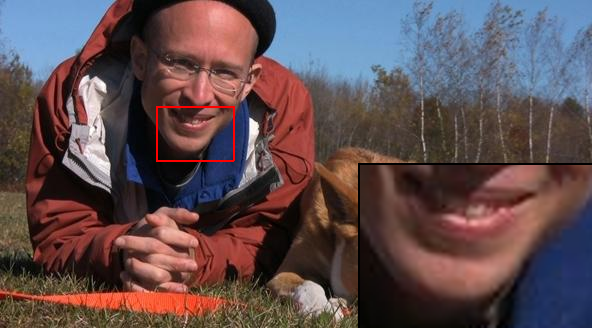
\includegraphics[width=0.24\textwidth]{dog[1-Original].png}&
% \hspace{-4.5mm} 
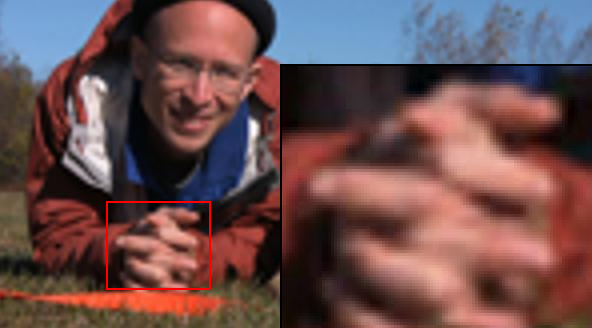
\includegraphics[width=0.33\textwidth]{MI/dog[2-Bicubic].png}&
\hspace{-4.5mm} 
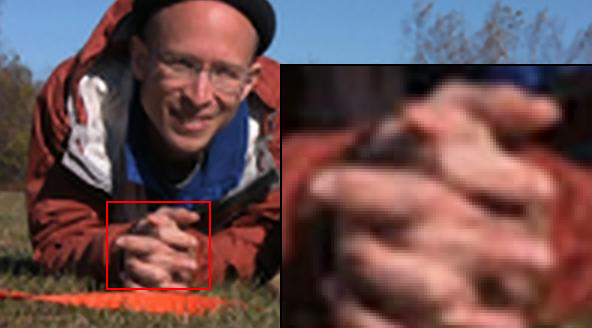
\includegraphics[width=0.33\textwidth]{MI/dog[3-JOR].png}&
\hspace{-4.5mm} 
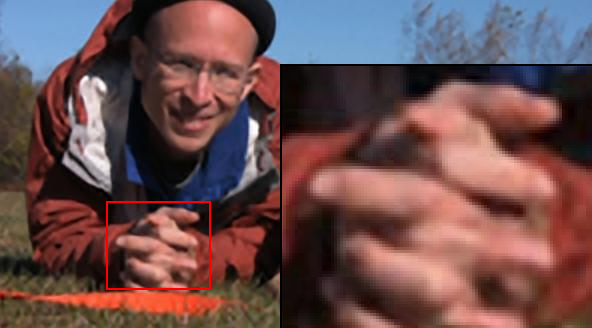
\includegraphics[width=0.33\textwidth]{MI/dog[4-JOR+MI].png}\\

% \hspace{-2mm}
% \includegraphics[width=0.24\textwidth]{street[1-Original].png}&
% \hspace{-4.5mm} 
% \includegraphics[width=0.24\textwidth]{street[2-Bicubic].png}& 
% \hspace{-4.5mm} 
% \includegraphics[width=0.24\textwidth]{street[3-JOR].png}&
% \hspace{-4.5mm} 
% \includegraphics[width=0.24\textwidth]{street[4-JOR+MI].png}\\


% \hspace{-2mm}
% 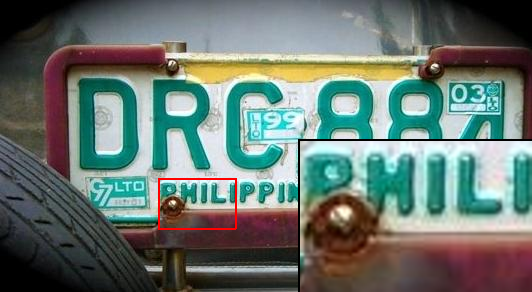
\includegraphics[width=0.24\textwidth]{license[1-Original].png}&
\hspace{-2mm} 
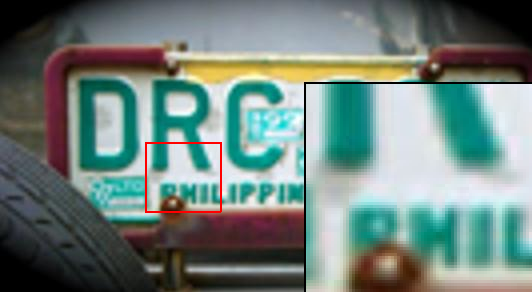
\includegraphics[width=0.32\textwidth]{MI/license[2-Bicubic].png}&
\hspace{-4.5mm} 
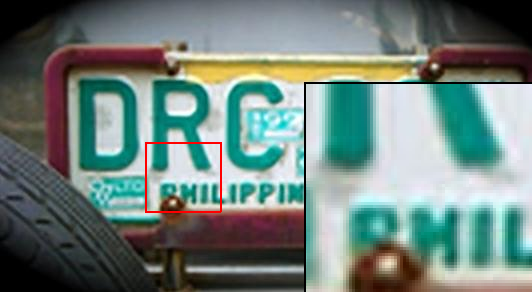
\includegraphics[width=0.32\textwidth]{MI/license[3-JOR].png}&
\hspace{-4.5mm} 
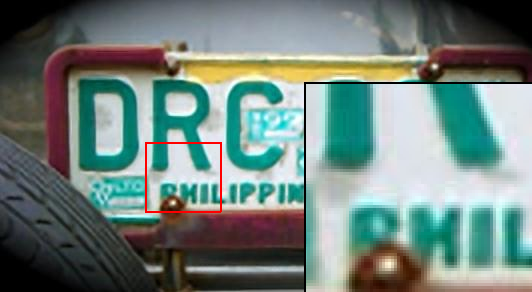
\includegraphics[width=0.32\textwidth]{MI/license[4-JOR+MI].png}\\
% \footnotesize{\text{Original}} & 
\footnotesize{\text{Bicubic}} & \footnotesize{\text{JOR}} & \footnotesize{\text{\textbf{JOR + MI}}} \\
\end{tabular}$
%}
%}
\caption{Examples with an upscaling factor $\times4$. Best seen on the
  screen. Images are obtained from the Internet.}
\label{fig:sr}
%\vspace{-0.5cm}
\end{figure*}


\subsection{Instance-based Object Retrieval}

MI was also tested for instance-based object retrieval, where the goal
is, given an object instance, to retrieve all instances of the same 
object class. The latter can be captured from different views, from different
distances, etc. We used the same features as for image clustering in 
Sec.\ref{sec:img:clustering}.

\textbf{Datasets}: Two of the most popular datasets for this task were
used: the INRIA Holidays dataset~\citep{hamming:embedding:08} and the
UKbench dataset~\citep{ukbench:cvpr06}. Holidays provides $500$ image
groups with $1,491$ images in total and for a very large variety of
scene types. Each group consists of photos of the same scene/object
taken under different conditions: rotations, viewpoint and
illumination changes. UKbench contains $10,200$ images of $2,550$
objects, $4$ images for each object from different views and distances.


\textbf{Results:} Half of the object classes (floored to closest integer) were used for training 
(to learn the mapping function) and the rest for testing. 
% For Holidays, MI was trained on the Scene-15 dataset
% (without using labels) as they both contain scene types. For UKbench,
% MI was trained on Caltech-101 (again without using labels), as both
% contain objects. 
MAP was again used as the criterion.  The results for
LBP are listed in Table~\ref{tab:retrieval}.  % The trends for GIST and
% PHOG are similar, as reported in the supplementary material.
It is interesting to see that even when trained on different datasets
without using any labels, MI is able to learn good metrics for object
retrieval. The learned metrics are significantly better than the
standard ones over the TFs. For instance, the MAP of LBP 
is improved from $0.38$ to $0.50$ on Holidays and from $0.33$ to
$0.44$ on the UKbench dataset, when the CNN feature is used as the SFs. Yet, there is still room for
improvement when compared against the performance of the
state-of-the-art object retrieval systems
(\eg~\citep{qin:bmvc14}). There are two main reasons: 1) MI is trained in a fully unsupervised manner:
trained on different objects and without using any human annotations; 2) MI uses cheap, low-dimensional features for
the sake of efficiency (the difference to \citep{qin:bmvc14} in terms
of feature dimensionality is as large as 3 orders of magnitude). The
goal of MI is different, i.e. providing an efficient solution and avoiding
any human annotations.

\subsection{Image Super-resolution}
The goal of image super-resolution is to generate high-resolution (HR) images from
low-resolution (LR) ones. Example-based learning methods have proven
successful in learning from a collection of patch pairs: LR patches
and corresponding HR patches~\citep{Chang-CVPR-2004, Timofte-ICCV-2013,
  Dong-ECCV-2014, JOR:EG15}. In this section, we apply MI to
example-based image super-resolution. In order to better show the
advantage of MI, we follow the approaches which are directly based on $k$-NN
search~\citep{Freeman-CGA-2002, Chang-CVPR-2004, JOR:EG15}. The very
recent method JOR~\citep{JOR:EG15} was employed for comparison. JOR
jointly learns a collection of regressors from LR patches to HR ones,
which collectively yield the smallest super-resolving error for all
training data, and selects the most appropriate regressor for each
test patch via a voting scheme by its $k$ nearest neighbors from the
training samples. MI replaces the standard $L_2$ metric in the $k$-NN
search by the learned metric, and keeps the rest of the system
intact.
% We build on top of
% ANR~\citep{Timofte-ICCV-2013}. During training, ANR partitions the
% space of all LR patches by placing anchors, and then associates each
% anchor with a regression function to project LR patches to HR
% ones. During test time, the nearest anchors of test-LR patches are
% computed by correlation, and the corresponding regression functions
% are used for patch up-scaling.  We replace the correlation-based
% metric by an MI-learned metric for searching the nearest anchors. The
% rest of the framework is kept the same.
By the replacement, the method (JOR + MI) is now trying (via imitation) to
retrieve neighbors defined over HR patches: searching for LR patches
whose corresponding HR patches are similar to the desired HR patch of
the test LR patch.  This exactly tallies with the goal of
example-based image super-resolution.


Since the number of training samples for image super-resolution is
much larger (often millions) than that for other vision tasks considered 
in this paper, solving the eigenvector problem of MI directly is 
intractable. We employed the eigenfunction technique~\citep{Fergus09} 
for an approximate solution.  We
tested MI with $0.5$ million training patches.  The method was
evaluated on the two standard datasets Set5 and Set14, and MI improves
the PSNR from $32.30$ to $32.53$ on Set5, and from $28.90$ to $29.10$
on Set14 for an upscaling factor of $\times 3$. For a factor $\times 4$,
MI improves JOR from $29.94$ to $30.15$ on Set5 and from $27.13$ to
$27.25$. The method JOR + MI trained with $0.5$ million patches is on
par with the JOR trained with $5$ million patches~\citep{JOR:EG15}, but
is considerably faster both at training and testing.  The method also
outperforms the very recent method SRCNN~\citep{Dong-ECCV-2014} using
deep convolutional network, in terms of both performance and speed (in
terms of speed at testing, SRCNN is on par with JOR trained from 5
million patches~\citep{JOR:EG15}). We also trained the
method with $5$ million patches, but observed no further improvement. 
A possible reason is that once samples densely cover
the space, standard metrics are sufficient to find good
neighbors. We leave the investment to learn more effectively from very large datasets as our future work. 
However, we believe that the case with $0.5$ million
patches suffices to prove the concept: MI yields an
efficient solution to image super-resolution without sacrificing 
performance. 
% from $28.65$ to $29.07$ on Set14 for a super-resolution scaling factor
% of $\times 3$, and from $29.69$ to $30.10$ on Set5 and from $26.85$ to
% $27.26$ on Set14 for a super-resolution scaling factor of $\times 4$.
Two image examples are shown in Fig.~\ref{fig:sr}. The examples and
the numbers show that MI improves the results of JOR by
transferring domain knowledge from the space of HR patches into that
of LR patches. 

\section{Conclusion}
\label{sec:con}
The paper proposed the novel Metric Imitation method to
learn good metrics for features in one domain (target
features, TFs) by imitating the metrics computed over features of
another domain (source features, SFs), and this even without supervision. 
MI translates the neighborhood
behavior of SFs into manifold geometry, and transfers it to the domain
of TFs as a guide for metric learning. MI then seeks a linear mapping
function of the TFs so that the transferred manifold can be
approximated well, which leads to an imitation of the metrics computed
over the SFs. The method is easy to understand and easy to implement. The usefulness
of MI has been corroborated by two scenarios with four popular vision
tasks. Extensive experiments have shown that MI is able to learn 
significantly better metrics over cheap TFs, while only slightly
increasing the time complexity during testing. We hope the idea of metric
imitation and manifold transfer will also prove useful for metric
learning and transfer learning. The code is available at
  \url{www.vision.ee.ethz.ch/~daid/MetricImitation}.
